\documentclass[10pt,a4paper]{article}
\usepackage[top=0in, bottom=0.5in,margin=1in, includefoot]{geometry}
\usepackage[utf8]{inputenc}
\usepackage[T1]{fontenc}

\title{Numerical analysis - Exercise 1}
\author{}
\date{}

\setlength\parindent{0pt}
\usepackage{amsmath}
\usepackage{wrapfig}
\usepackage{graphicx}
\usepackage{lineno}
\usepackage{layout}
\setlength{\voffset}{-0.4in}
\textheight = 735pt
\begin{document}
\vspace{-20mm}
\title{\textbf{EE2-08C Numerical Analysis} \\ Group 9\vspace{-17mm}}
\maketitle

\section*{Exercise 1}\vspace{-1mm}

\begin{wrapfigure}{r}{0.5\textwidth}
\vspace{-10mm}
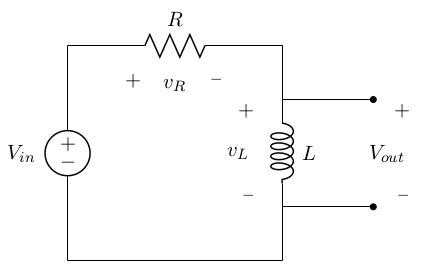
\includegraphics[width=0.49\textwidth]{RL_circuit.png}
\vspace{-6mm}
\caption{RL Circuit}
\label{fig:RL}
\end{wrapfigure}

This simple RL circuit forms a high pass filter circuit which takes an input signal Vin and only allows the high frequency components to pass. Despite the inductor being less convenient than a capacitor, this RL circuit can approach the model of a DC motor. In this specific case, we want to model a DC motor with inertia 250 $\mu$sNm/s$^2$ and $T_{max} = 50mNm/A$. To do so, according to KCL, we know that
\[Vin(t) = v_L(t) + v_R(t)\]

and therefore:

\[ V_{in}(t) = L\frac{d}{dt}i_L(t) + R i_L(t) \]

$i_L(t)$ is the state that we will solve following the three different second-order Runge Kutta methods.

All methods follow the same pattern:

\[x_{i+1} = x_i + h\]
$h$ being the step size and
\[y_{i+1} = y_i + h (a k_1 + b k_2)\]

where

\[k_1 = f(x_i, y_i)\]
\[k_2 = f(x_i + p h, y_i + q k_1 h)\]

and the values of $a, b, p$ and $q$ depend on which method we are using:

\begin{center}
 \begin{tabular}{||c | c c c||}
 \hline
 Parameter & Heuns & Midpoint & Ralston \\ [0.5ex]
 \hline\hline
 a & 1/2 & 0 & 1/4 \\
 \hline
 b & 1/2 & 1 & 3/4 \\
 \hline
 p & 1 & 1/2 & 2/3 \\
 \hline
 q & 1 & 1/2 & 2/3 \\ [1ex]
 \hline
\end{tabular}
\end{center}

Each method will approximate the exact solution according to these parameters. Therefore, the smaller the step size $h$, the more exact the method will approximate the solution.

 After doing so, the output value will be obtained as follows:

\[V_{out} = V_{in}(t) - R i_L(t)\]



\end{document}
